%Matteo Kumar - Leonard Schatt
% Fortgeschrittenes Physikalisches Praktikum
 
\section{Crystalls and Symmetry}\label{sec:Q4}

Crystalls can be found as whole or parts of minerals of natural products such as sugars, vitamins, proteins and many more~\cite{Bohm.2021}. They are defined as solid states which show a three dimensional periodic repitition of a pattern of atoms on a microscopic level. This pattern can be isotropic or anisotropic~\cite{Schwarzenbach.2001}. Knowing the crystal structure allows a description of its macroscopic structure and physical properties. A essential property of a crystal is its symmetry. Symmetry as such describes a periodic recurrance of a motive, not necessarily in space, but also e.g.~in time. In crystals, symmetry operations are a combination of mirror symmetry, radial symmetry and inversion. Cubic symmetry is one class of symmetry, which combines several symmetries, as can be seen in fig.~\ref{fig:CubeSymm}. A cube has three four-fold axes (through the middle of two opposite sides), four three-fold axes (through to opposite corners), six two-fold axes (through the middle of two opposite corners), nine mirroring planes (one perpendicular to every four- and two-fold axis) and one inversion centre~\cite{Bohm.2021}. The repetition unit of a cubic lattice is defined through three vectors $\mathbf{a}$, $\mathbf{b}$ and $\mathbf{c}$ with $|\mathbf{a}|=|\mathbf{b}|=|\mathbf{c}|$ and $\alpha = \beta = \gamma =$ \SI{90}{\degree}~\cite{Schwarzenbach.2001}. There are three types of cubic Bravais lattices: simple cubic (sc), body centered cubic (bcc) and face centered cubic (fcc) as can be seen in fig~\ref{fig:ScBccFcc}. The positions of the atoms are described by the basis, which can be identical to the vectors describing the lattice, but need not to. For instance, the positions of the atoms of zinc blende $ZnS$ are described by a fcc lattice and basis vectors (0,0,0) and (0.25,0.25,0.25) (see fig.~\ref{fig:ZnSStructure}).

\begin{figure}[ht]
    \centering
    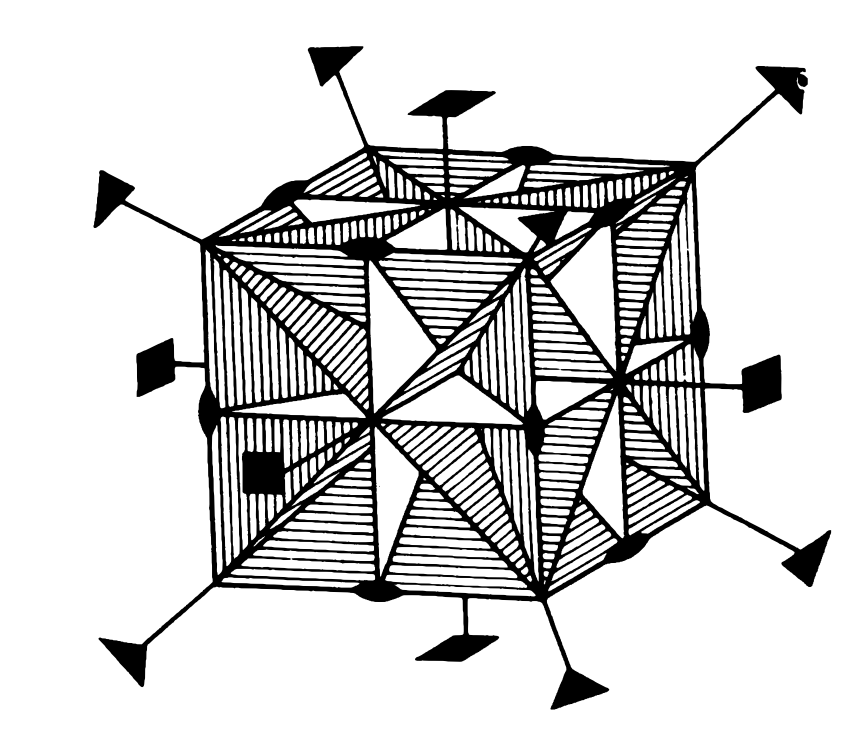
\includegraphics[width = 0.45\linewidth]{Bilder/Grundlagen/cube symmeries.png}
    \caption{A cube is a highly symmetric body. It has several mirroring and rotation axes aswell as an inversion center. Figure from~\cite{Bohm.2021}.}
    \label{fig:CubeSymm}
\end{figure}

\begin{figure}[ht]
    \centering
    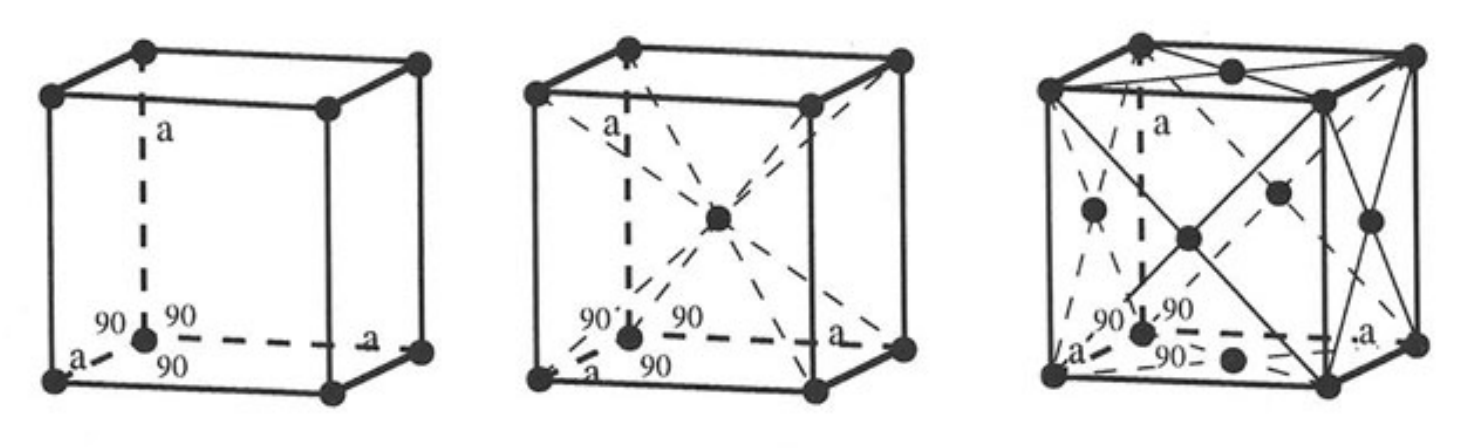
\includegraphics[width = 0.8\linewidth]{Bilder/Grundlagen/cubic lattices.png}
    \caption{The three types of cubic lattices: simple cubic (sc), body centered cubic (bcc) and face centered cubic (fcc). Figure from~\cite{Schwarzenbach.2001}}
    \label{fig:ScBccFcc}
\end{figure}

\begin{figure}[ht]
    \centering
    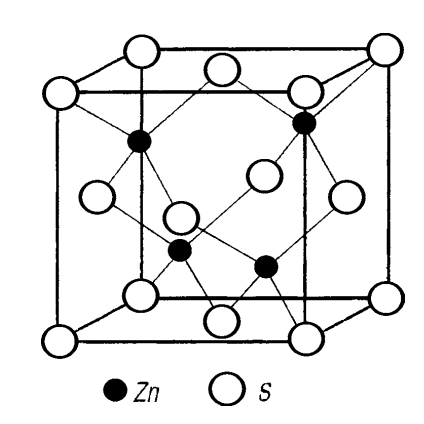
\includegraphics[width = 0.45\linewidth]{Bilder/Grundlagen/ZnS.png}
    \caption{Unit cell of a $ZnS$ structure. It is basically a fcc structure, but has a two atom basis: The $Zn$ atom is at (0,0,0) and the $S$ atom is at (0.25,0.25,0.25). Figure from~\cite{Bohm.2021}}
    \label{fig:ZnSStructure}
\end{figure}